
\section{Conclusions}
For large complex graphs, visual analytics may not form a suitable solution. Instead, it is possible to apply a range of mathematical algorithms to tell us what species are important within a network. Chemical mechanisms, much like many real-world graphs, were shown to have both small world and scale-free properties within their structure. This means that they have both a local(social) and global(hierarchical) structure. 

It was shown that it is possible to generate a citation network for papers citing the master chemical mechanism and represent this in the form of a graph. Further exploration into the network structure led to the creation of a co-citation and an author network from the original dataset. This was then used to evaluate several centrality metrics, and their ability to highlight roles within the co-authorship network. 

Next, the centrality metrics were applied to a range of chemical mechanisms representing urban, terrestrial and marine environments. Here it was seen that the sum of these follows a similar trend to more traditional methods of evaluating node importance, such as flux and concentration analysis. As this was the case, averaged metric values for each scenario were generated, and the individual chemistry compared with the aid of a TF-IDF algorithm. This highlights important species for each run, whilst ignoring those which are important across all runs.

Finally, it was noted that in reversing the direction of links within a graph it is possible to determine the source of influence on a node. An attempt to do this using the PageRank algorithm was made, although this proved to not be the most effective method to accomplish this. Instead, it was far simpler to make use of the adjacency matrix (jacobian) and apply the transformation there to get the required results. 

In this chapter the merit of using centrality metrics to mathematically analyse a complex network was shown. It is suggested that these are used in conjunction with more traditional methods of simulation evaluation to allow for a greater understanding of the roles each species have within a certain environment. 

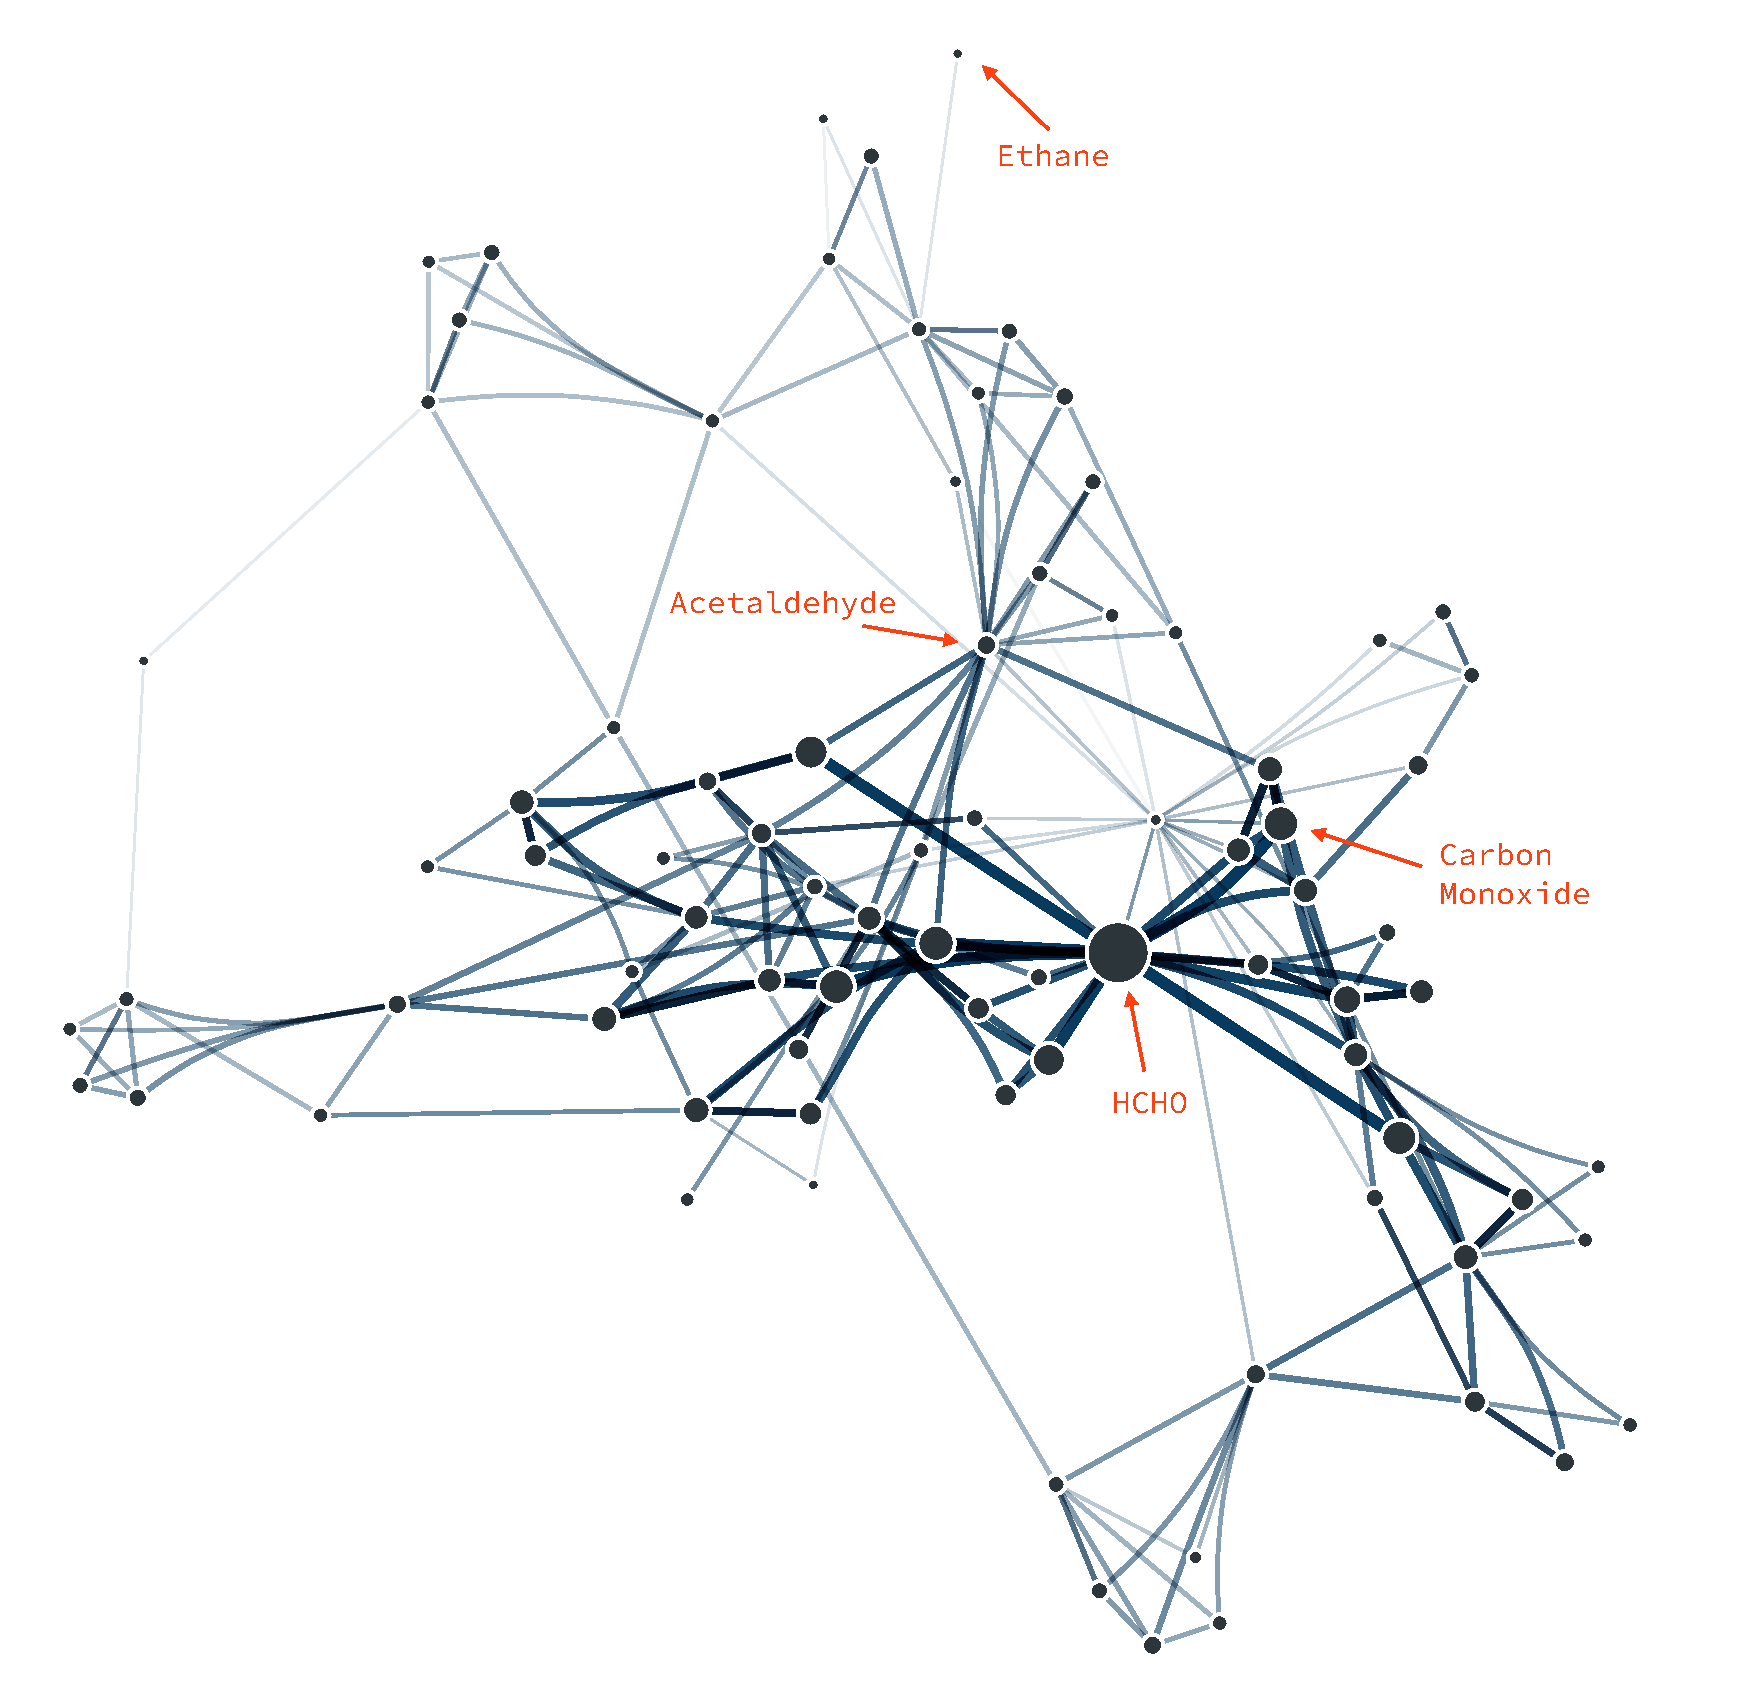
\includegraphics[width=\textwidth]{figures_c3/ch2_distance.pdf}